\documentclass[12pt]{IEEEtran}
\IEEEoverridecommandlockouts
\usepackage{fancyhdr}
\usepackage{graphicx}
\usepackage[spanish, es-tabla, es-nodecimaldot]{babel}
% \usepackage[utf8]{inputenc}
\usepackage{csquotes}
\usepackage{wrapfig}
\usepackage[l3]{csvsimple}
\usepackage{array}
\usepackage[calc, spanish]{datetime2}
\usepackage{enumitem}
% \usepackage{multicol}
\usepackage{chemformula}
\usepackage{multirow}
\usepackage{mismath}
\usepackage{adjustbox}
\usepackage{nccmath}
\usepackage{amsmath}
\usepackage{amssymb}
\usepackage{mathtools}
\usepackage{amsfonts,latexsym} % para tener disponibilidad de diversos simbolos
\usepackage{enumerate}
\usepackage{empheq}
\usepackage{derivative}
\usepackage{float}
\usepackage{threeparttable}
\usepackage{ifpdf}
\usepackage{rotating}
\usepackage{stfloats}
\usepackage{tabularray}
\usepackage{url}
% \usepackage[inline]{showlabels}
\usepackage{kantlipsum}
\usepackage{siunitx}
\usepackage{makecell}%To keep spacing of text in tables
\setcellgapes{2pt}%parameter for the spacing in tables
\usepackage{afterpage}
\usepackage{subcaption}
\usepackage[
  sorting=none,
  backend=biber,
  style=ieee,
  % bibstyle = authoryear,
  citestyle=numeric-comp,
]{biblatex}
\usepackage{hyperref}
\usepackage{cleveref}
\crefname{table}{tabla}{tablas} % Table's cross-reference name
\crefname{equation}{ec.}{ecs.} %
\newcommand\crefrangeconjunction{--}
\newcommand\crefpairconjunction{~y~}
\providecommand{\abs}[1]{\lvert#1\rvert}
%%%%%%%%%%%%%%%%%%%%%%%%%%%%%%%%%%%%%%%%%%%
%%% CREAR Y REESCRIBIR ALGUNOS COMANDOS %%%
%%%%%%%%%%%%%%%%%%%%%%%%%%%%%%%%%%%%%%%%%%%
\newcolumntype{P}[1]{>{\centering\arraybackslash}p{#1}}  %% Se crea un nuevo tipo de columna llamada P.
\newcommand{\tabitem}{~~\llap{\textbullet}~~}
\newcommand{\ctt}{\centering\scriptsize\textbf} %%\ctt abrevia el comando \centering\scriptsize\textbf
\newcommand{\dtt}{\scriptsize\textbf} %%\dtt abrevia el comando \scriptsize\textbf
\renewcommand\IEEEkeywordsname{Palabras clave}

%% Crea una lista en dos columnas
\SetEnumitemKey{twocol}{%
  itemsep = 1\itemsep,
  parsep = 0.5\parsep,
  before = \raggedcolumns
  \begin{multicols}{2},
    after =
\end{multicols}}
%%%%%%%%%%%%%%%%%%%%%%%%%%%%%%%%%%%%%%%%%%%

% correct bad hyphenation here
\hyphenation{op-tical net-works semi-conduc-tor} %% Con este comando se especifican como pueden seprarse las sílabas adecuadamente en caso una palabra quede en dos lineas diferentes de texto

\graphicspath{ {figs/} {logos/}}  %%Ruta donde se encuentran las imágenes, que esté vacio indica que las imagenes están dentro de la misma carpeta que contiene el archivo .tex

\sisetup{
  output-decimal-marker = {.},
  uncertainty-mode = separate,
}
% adjust as needed
\addtolength{\footskip}{0\baselineskip}
\addtolength{\textheight}{-1\baselineskip}

%Paquete tikz para hacer diagramas y figuras
\usepackage{tikz}
\usetikzlibrary{arrows}
%\usepackage[spanish,es-noquoting]{babel}

\DeclareSIUnit{\Torr}{Torr}
\DeclareSIUnit{\mTorr}{mTorr}

%%%%%%%%%%%%%%%%%%%%%%%%%%%%%%%%
%%%%% INICIO DEL DOCUMENTO %%%%%
%%%%%%%%%%%%%%%%%%%%%%%%%%%%%%%%

\addbibresource{CaracterizacionPeliculaDelgadaAluminioHiPIMSTribologia.bib}

\DTMsavedate{duedate}{2024-03-25}% Año-Mes-Día -> Fecha de entrega
\DTMnewdatestyle{usvardate}{%
  \renewcommand{\DTMdisplaydate}[4]{%
    \DTMMonthname{##2}\nobreakspace% Mes
    \number##1% Año
  }%
  \renewcommand{\DTMDisplaydate}{\DTMdisplaydate}%
}

\DeclareSIUnit{\min}{min}

\begin{document}
%%%%%%%%%%%%%%%%%%%%%%%%%%%%
%%% TÍTULO DEL DOCUMENTO %%%
%%%%%%%%%%%%%%%%%%%%%%%%%%%%

\title{Estudio de películas delgadas de \ch{Al} depositadas por High-Power Impulse Magnetron Sputtering}

%%%%%%%%%%%%%%%%%%%%%%%%%%%
%%%%%%%%% AUTORES %%%%%%%%%
%%%%%%%%%%%%%%%%%%%%%%%%%%%

\author{\IEEEauthorblockN{Jesús Diego Gómez Garnica, Marcos López Merino}\\
	\IEEEauthorblockA{\textbf{Profesor}: Julio César Cruz Cárdenas}\\
	\IEEEauthorblockN{\DTMusedate{duedate}}}

%%%%%%%%%%%%%%%%%%%%%%%%%%%
\twocolumn[
	\begin{@twocolumnfalse}
		\maketitle
		\begin{abstract}
			Las películas delgadas de \ch{Al} tienen aplicaciones en dispositivos electrónicos, almacenamiento de energía y recubrimientos protectores. Con el objetivo de estudiar la adherencia y morfología de películas de \ch{Al}, se depositaron sobre sustratos de vidrio y silicio \ch{Si} mediante High-Power Impulse Magnetron Sputtering (HiPIMS). Las películas se caracterizaron mediante perfilometría óptica (OP), microscopía electrónica de barrido (SEM) y pruebas de \emph{scratch} (\emph{Single Point Scratch Testing}). Los resultados mostraron un espesor promedio de \qty{280}{\nm}. Las pruebas de \emph{scratch} revelaron una carga crítica de \qty{0.1}{\N} y \qty{0.5}{\N}, sugiriendo problemas de adherencia. Estos resultados subrayan la de técnicas complementarias para una caracterización adecuada de las películas de \ch{Al} depositadas por esta técnica.
		\end{abstract}

		\begin{IEEEkeywords}
			HiPIMS, SEM, Scratch Test
		\end{IEEEkeywords}
	\end{@twocolumnfalse}
	\vspace{1cm}
]

%https://doi.org/10.1016/j.surfcoat.2022.128409 -> Aplicaciones

%%%%%%%%%%%%%%%%%%%%%%
%\IEEEpeerreviewmaketitle
%%%%%%%%%%%%%%%%%%%%%%%%%%%%%%%%%%%%%
%%% PRIMERA SECCIÓN DEL DOCUMENTO %%%
%%%%%%%%%%%%%%%%%%%%%%%%%%%%%%%%%%%%%
\section{Introducción}
Las películas delgadas son capas de uno o más materiales con espesores que van desde unos cuantos nanómetros hasta varios micrómetros. Estas pueden encontrarse en aplicaciones tan diversas como revestimientos antirreflejantes para anteojos o componentes funcionales en chips de computadoras. Su ventaja radica en la combinación de las propiedades superficiales de la película delgada con las propiedades del material subyacente, lo que mejora las características químicas, mecánicas o eléctricas, entre otras.
Existen múltiples técnicas para producir películas delgadas, tales como electrodeposición (\emph{electroplating}), la evaporación, la pulverización catódica (\emph{sputter deposition}), la deposición química de vapor  (CVD, por sus siglas en inglés) y combinaciones de estas. En este trabajo nos enfocaremos en una técnica recientemente desarrollada llamada \emph{high-power impulse magnetron sputtering} (HiPIMS) \cite{lundinHiPIMSProcess2010}.

HiPIMS es un método de deposición física de vapor (\emph{physical vapor deposition}, PVD) basado en la pulverización catódica con magnetrón de corriente directa (\emph{direct current magnetron sputtering}, DCMS). Esta técnica emplea densidades de potencia extremadamente altas, del orden de \unit{\kW\per\cm^{2}}, aplicadas en pulsos cortos de decenas de microsegundos. El plasma de HiPIMS se genera mediante una descarga luminiscente en la que la densidad de corriente puede alcanzar varios \unit{\A\per\squared\cm}, mientras que el voltaje de descarga se mantiene del orden de varios cientos de volts. Inicialmente, la descarga se distribuye de manera homogénea sobre la superficie del cátodo (blanco), pero al superar cierto umbral de densidad de corriente, esta se concentra en zonas de ionización que se desplazan a lo largo de una trayectoria conocida como \emph{racetrack} o camino de erosión. Este tipo de descarga se opera típicamente en modo pulsado, con ciclos de trabajo bajos, con el fin de evitar el sobrecalentamiento del blanco y otros componentes del sistema. En cada pulso, la descarga atraviesa varias etapas: ruptura eléctrica, plasma de gas, plasma metálico y un estado estacionario, que puede alcanzarse si el plasma metálico domina sobre el plasma de gas. Las películas obtenidas mediante HiPIMS suelen ser más densas y de mayor calidad en comparación con las producida por técnicas convencionales de pulverización catódica.

Las películas delgadas pueden caracterizarse mediante diversas técnicas para evaluar su crecimiento, calidad, entre otras características. Una de estas es la microscopía electrónica de barrido (\emph{scanning electron microscopy}, SEM), que emplea un haz enfocado de electrones para escanear la superficie de una muestra punto por punto y examinarla con alta resolución.

La interacción del haz de electrones con la superficie de la muestra da lugar a dos tipos distintos de electrones: electrones retrodispersados (\emph{backscattered electrons}, BSE) y electrones secundarios (SE). Los BSE son electrones de alta energía provenientes del haz incidente del SEM que experimentan dispersión elástica con los núcleos atómicos de la muestra. En contraste, los SE son electrones de bajas energías emitidos desde la superficie cuando es irradiada con el haz de electrones, el cual transfiere su energía a los electrones atómicos a través de colisiones inelásticas que se emiten desde los primeros nanómetros de la superficie de la muestra debido a su limitada profundidad de penetración \cite{WhichElectronDetector2023,infoInterpretingImagesScanning2022}.
Mediante la amplificación de la señal, es posible obtener imágenes topográficas de la superficie de la muestra con facilidad. Además, se pueden obtener imágenes de la sección transversal, lo que permite analizar tanto el espesor de la película como su microestructura.

Una prueba para evaluar las características mecánicas es la prueba de rayado (\emph{scratch}), en la que un contracuerpo (\emph{stylus}), se pone en contacto con la película. La muestra se coloca sobre una plataforma de alta precisión que la pone en contacto con la punta, moviéndola a una velocidad constante y aplicando una carga constante o progresiva. Se trata de una prueba tribológica empleada para evaluar la integridad mecánica, los modos de falla y la fuerza de adherencia del recubrimiento \cite{internationalStandardTestMethod}.

\begin{figure}[htp]
	\centering
	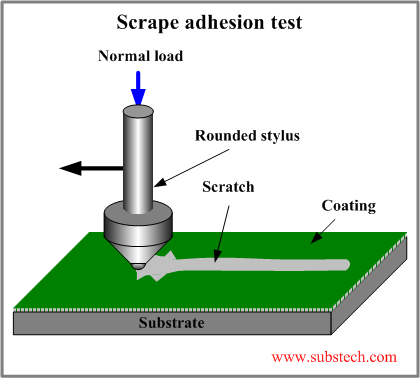
\includegraphics[width=0.8\linewidth]{scratch-test}
	\caption{Esquema de una prueba de rayado. \cite{kopeliovich_adhesion_nodate}}
	\label{fig:scratch-test}
\end{figure}

\section{Procedimiento experimental}

Mediante pruebas tribológicas se caracterizaron las películas delgadas de \ch{Al} depositadas en sustratos de \ch{Si} y portaobjetos de vidrio por la técnica de HiPIMS. Es necesario que se tomen las precauciones necesarias para evitar la contaminación de la muestras, ya que esto puedo afectar los resultados obtenidos.

\subsection{Medición del espesor}

Para la medición del espesor de las películas se requirió colocar una gota de pegamento en alguno de los sustratos, en particular, el portaobjetos de vidrio. Posteriormente, se retiró el pegamento y mediante la técnica de perfilometría óptica se midió el espesor en distintas áreas del cráter generado alrededor de ésta. El perfilómetro óptico utilizado fue el Nexview de la marca ZYGO.

\subsection{Prueba de \emph{scratch}}

La prueba de \emph{scratch} se realizó usando el tester mecánico NANOVEA CB500 para la película depositada en el portaobjetos de vidrio siguiendo la norma ASTM-1624\cite{internationalStandardTestMethod}. Esta se prueba se llevó acabo a una temperatura \qty{22.7}{\degreeCelsius} utilizando un contracuerpo de hierro con cromo de \qty{1}{\mm} aplicando una carga progresiva de \qty{0.01}{\N} hasta \qty{2.5}{\N} y de \qty{0.01}{\N} hasta \qty{1}{\N} con una velocidad constante de \qty{1}{\mm\per\min} en una distancia de \qty{5}{\mm}. Posteriormete se analizaron ambas trayectorias en el perfilómetro óptico en conjunto con el \emph{scratch test ATLAS} para caracterizar el tipo de cargas críticas en cada una de las pruebas.

\subsection{SEM}

El análisis de la morfología y el tipo de creciminento de la película delgada se realizó para la película depositada en el sustrato de \ch{Si} mediante un microscopio electrónico de barrido (SEM) de la marca JEOL, modelo JSM-6010LA. La imagen de la sección transversal se obtuvo utilizando usando SE a una resolución de \num{10000} y \num{20000}, y con BE a una resolución de \num{20000}. Mientras que la imagen para determinar el tipo de crecimiento se obtuvo usando solamente SE a resoluciones de \num{10000} y \num{25000}.

\section{Resultados y análisis}

A partir de las distintas mediciones realizadas con el perfilómetro óptico a lo largo del cráter, se determinó que el espesor de la película varía entre \qty{250}{\nm} y \qty{300}{\nm}, resultado el espesor en promedio de \qty{280}{\nm}. Esta variación es un indicio de que la pellícula depositada es amorfa y, aunque el depósito fue exitoso, sugiere que aún es necesario ajustar los parámetros utilizados durante el proceso: una presión base de \qty{3e-6}{\Torr}, presión de trabajo de \qty{10.7}{\mTorr}, frecuencia de \qty{90}{\Hz} (90 pulsos por segundo) durante \qty{25}{\min}, potencia de \qty{25}{\W}, voltaje de \qty{550}{\V} y corriente de \qty{14}{\mA}. En la \cref{fig:OP-grosor} se midió que el espesor en esa zona del cráteer generado por la presencia del pegamento era de \qty{280}{\nm}.

\begin{figure}[htp]
	\centering
	\includegraphics[width=0.8\linewidth]{OP-grosor}
	\caption{Medición del espesor de la película de \ch{Al} depositada en el portaobjetos de vidrio.}
	\label{fig:OP-grosor}
\end{figure}

Por otro lado, es necesario mencionar que la resolución del SEM utilizado para la obtención de las imágenes de la sección transversal y la superficie de la película de \ch{Al} depositada en el sustrato de \ch{Si} no fue la adecuada para observar la morfología y el tipo de crecimiento de la película. En la \cref{fig:SEM-trans} se observa la imagen de la sección transversal de la película, donde se puede observar que el cremiento es irregular y no uniforme, lo que sugiere que la película es amorfa. Mientras que en la \cref{fig:SEM-superficie} se observa la imagen de la superficie de la película, donde se puede observar que el crecimineto es granular.

\begin{figure*}[ht]
	\centering
	\begin{subfigure}[b]{0.45\textwidth}
		\centering
		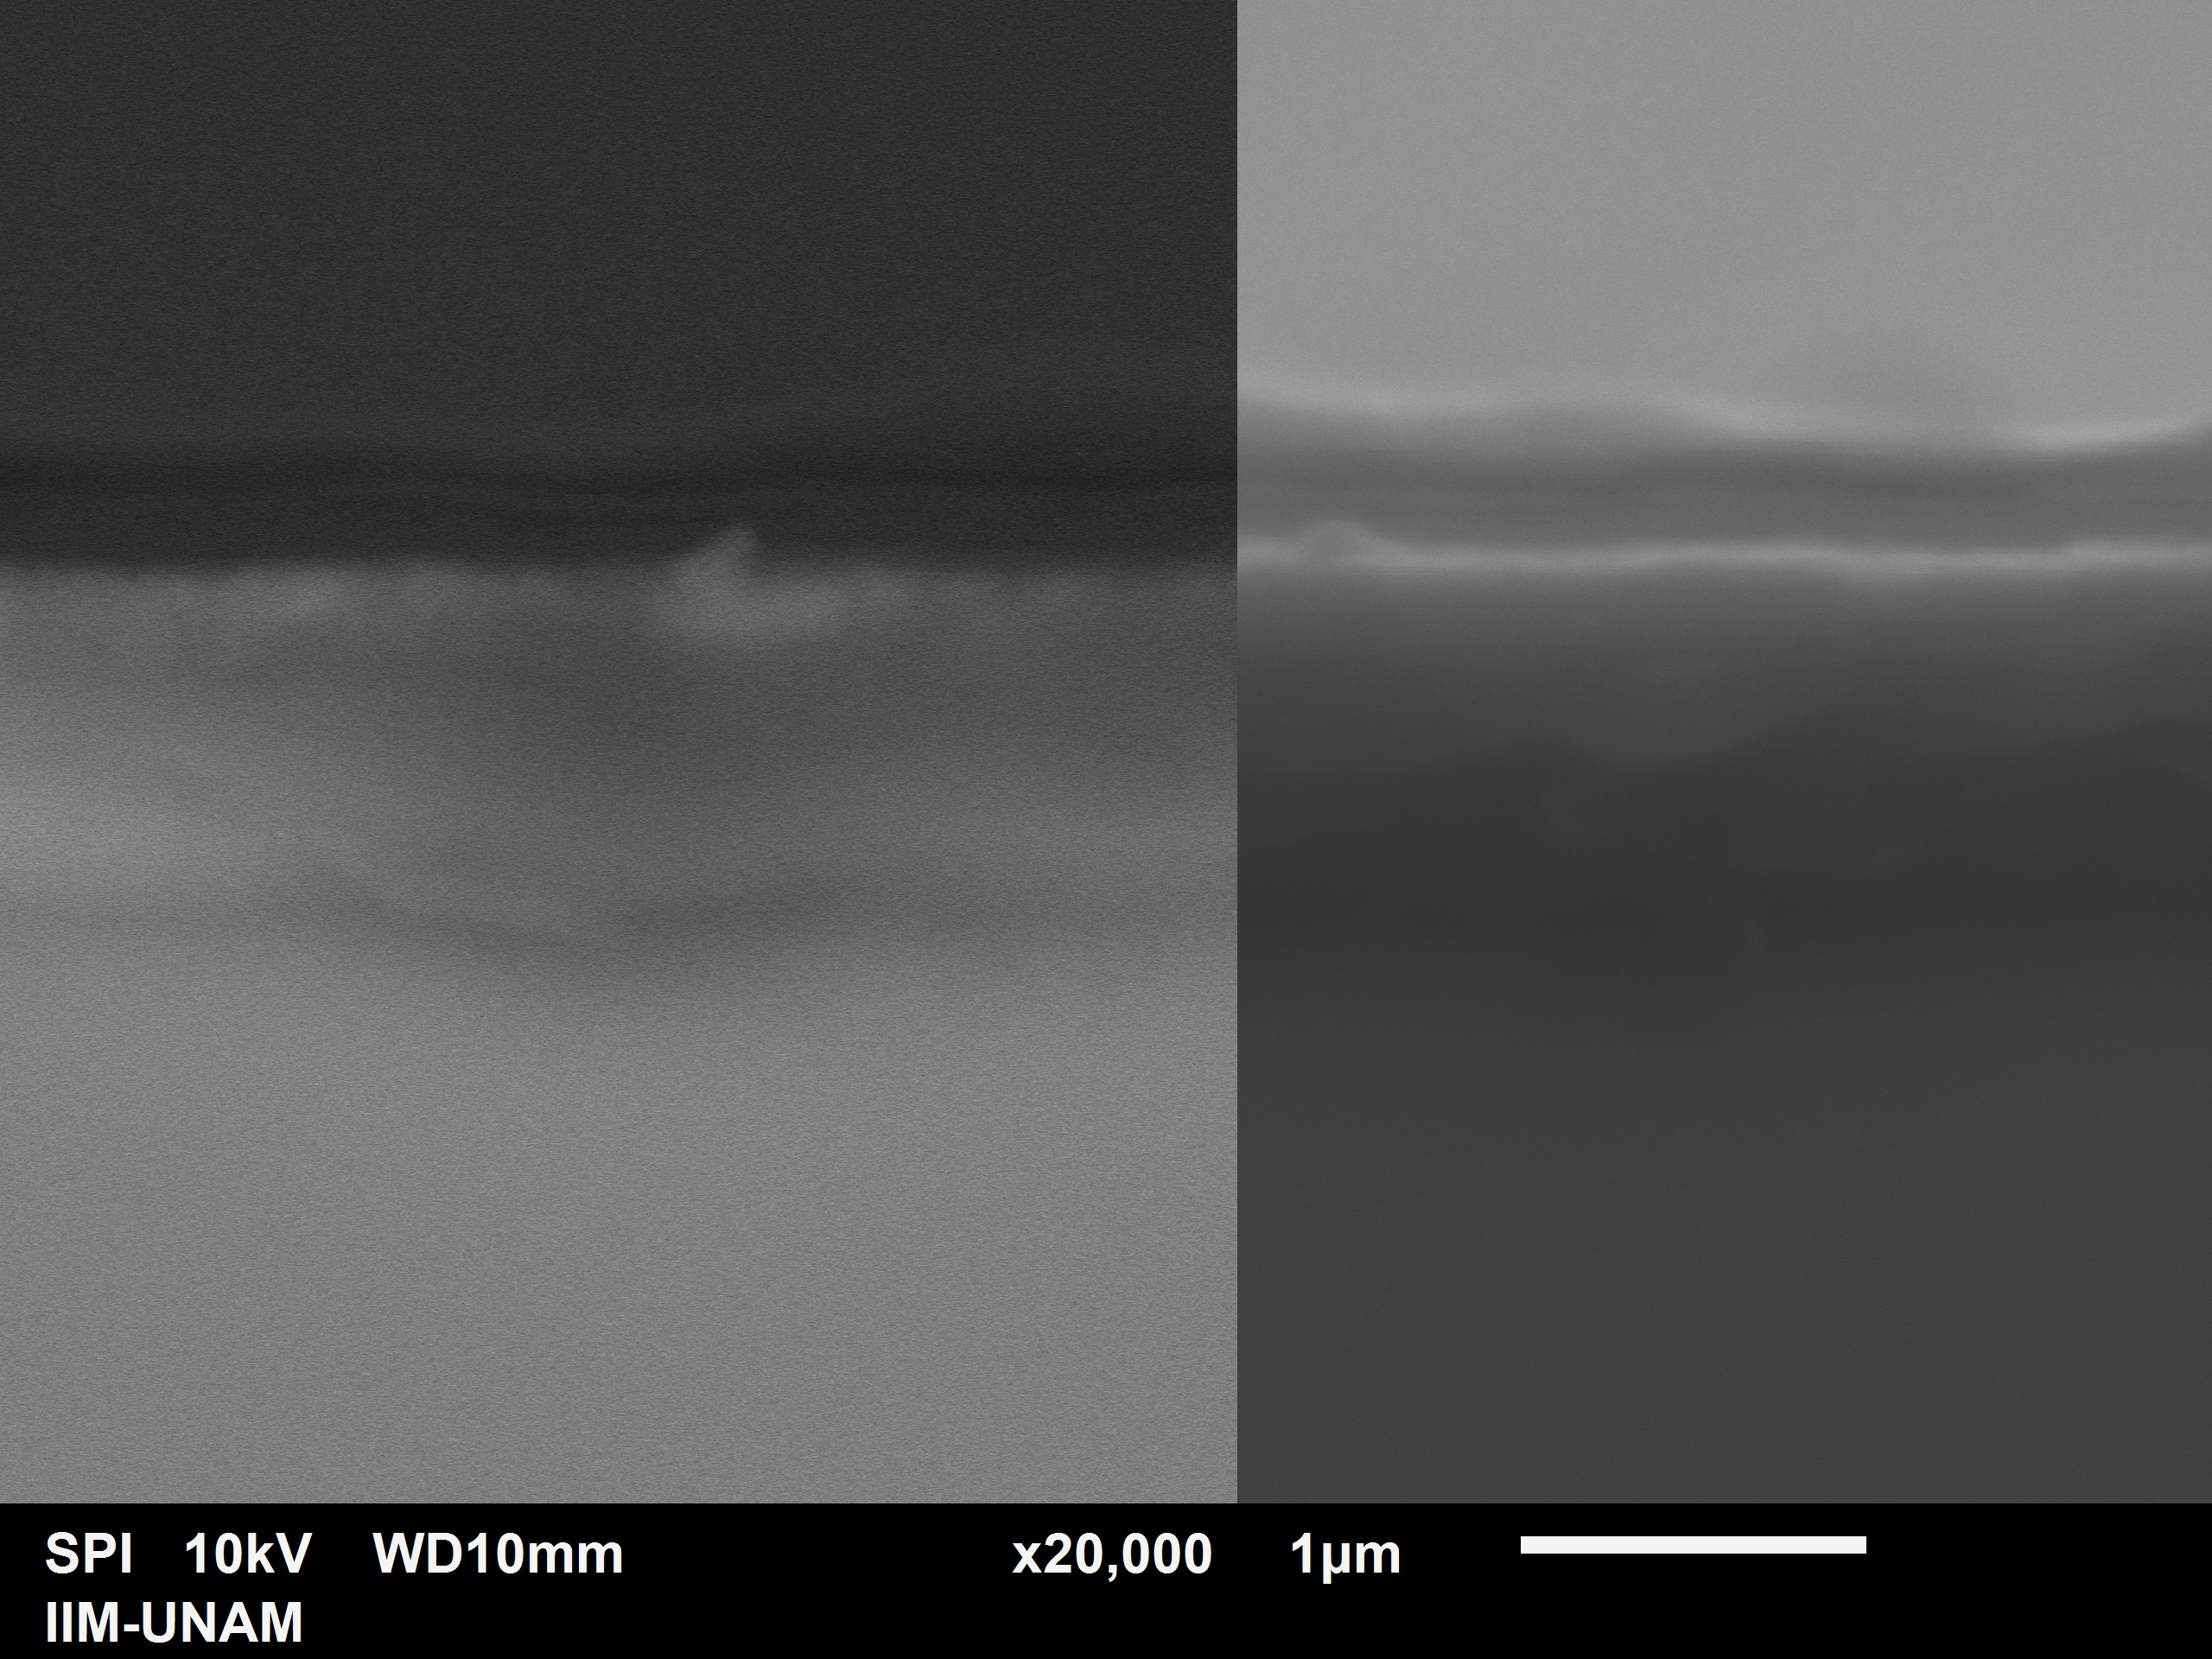
\includegraphics[width=\linewidth]{Al-transv-0004.png}
		\caption{Imagen de la sección transversal de la película de \ch{Al} depositada en el sustrato de \ch{Si}, con BSE a la izquierda y SE a la derecha.}
	\end{subfigure}%
	~
	\begin{subfigure}[b]{0.45\textwidth}
		\centering
		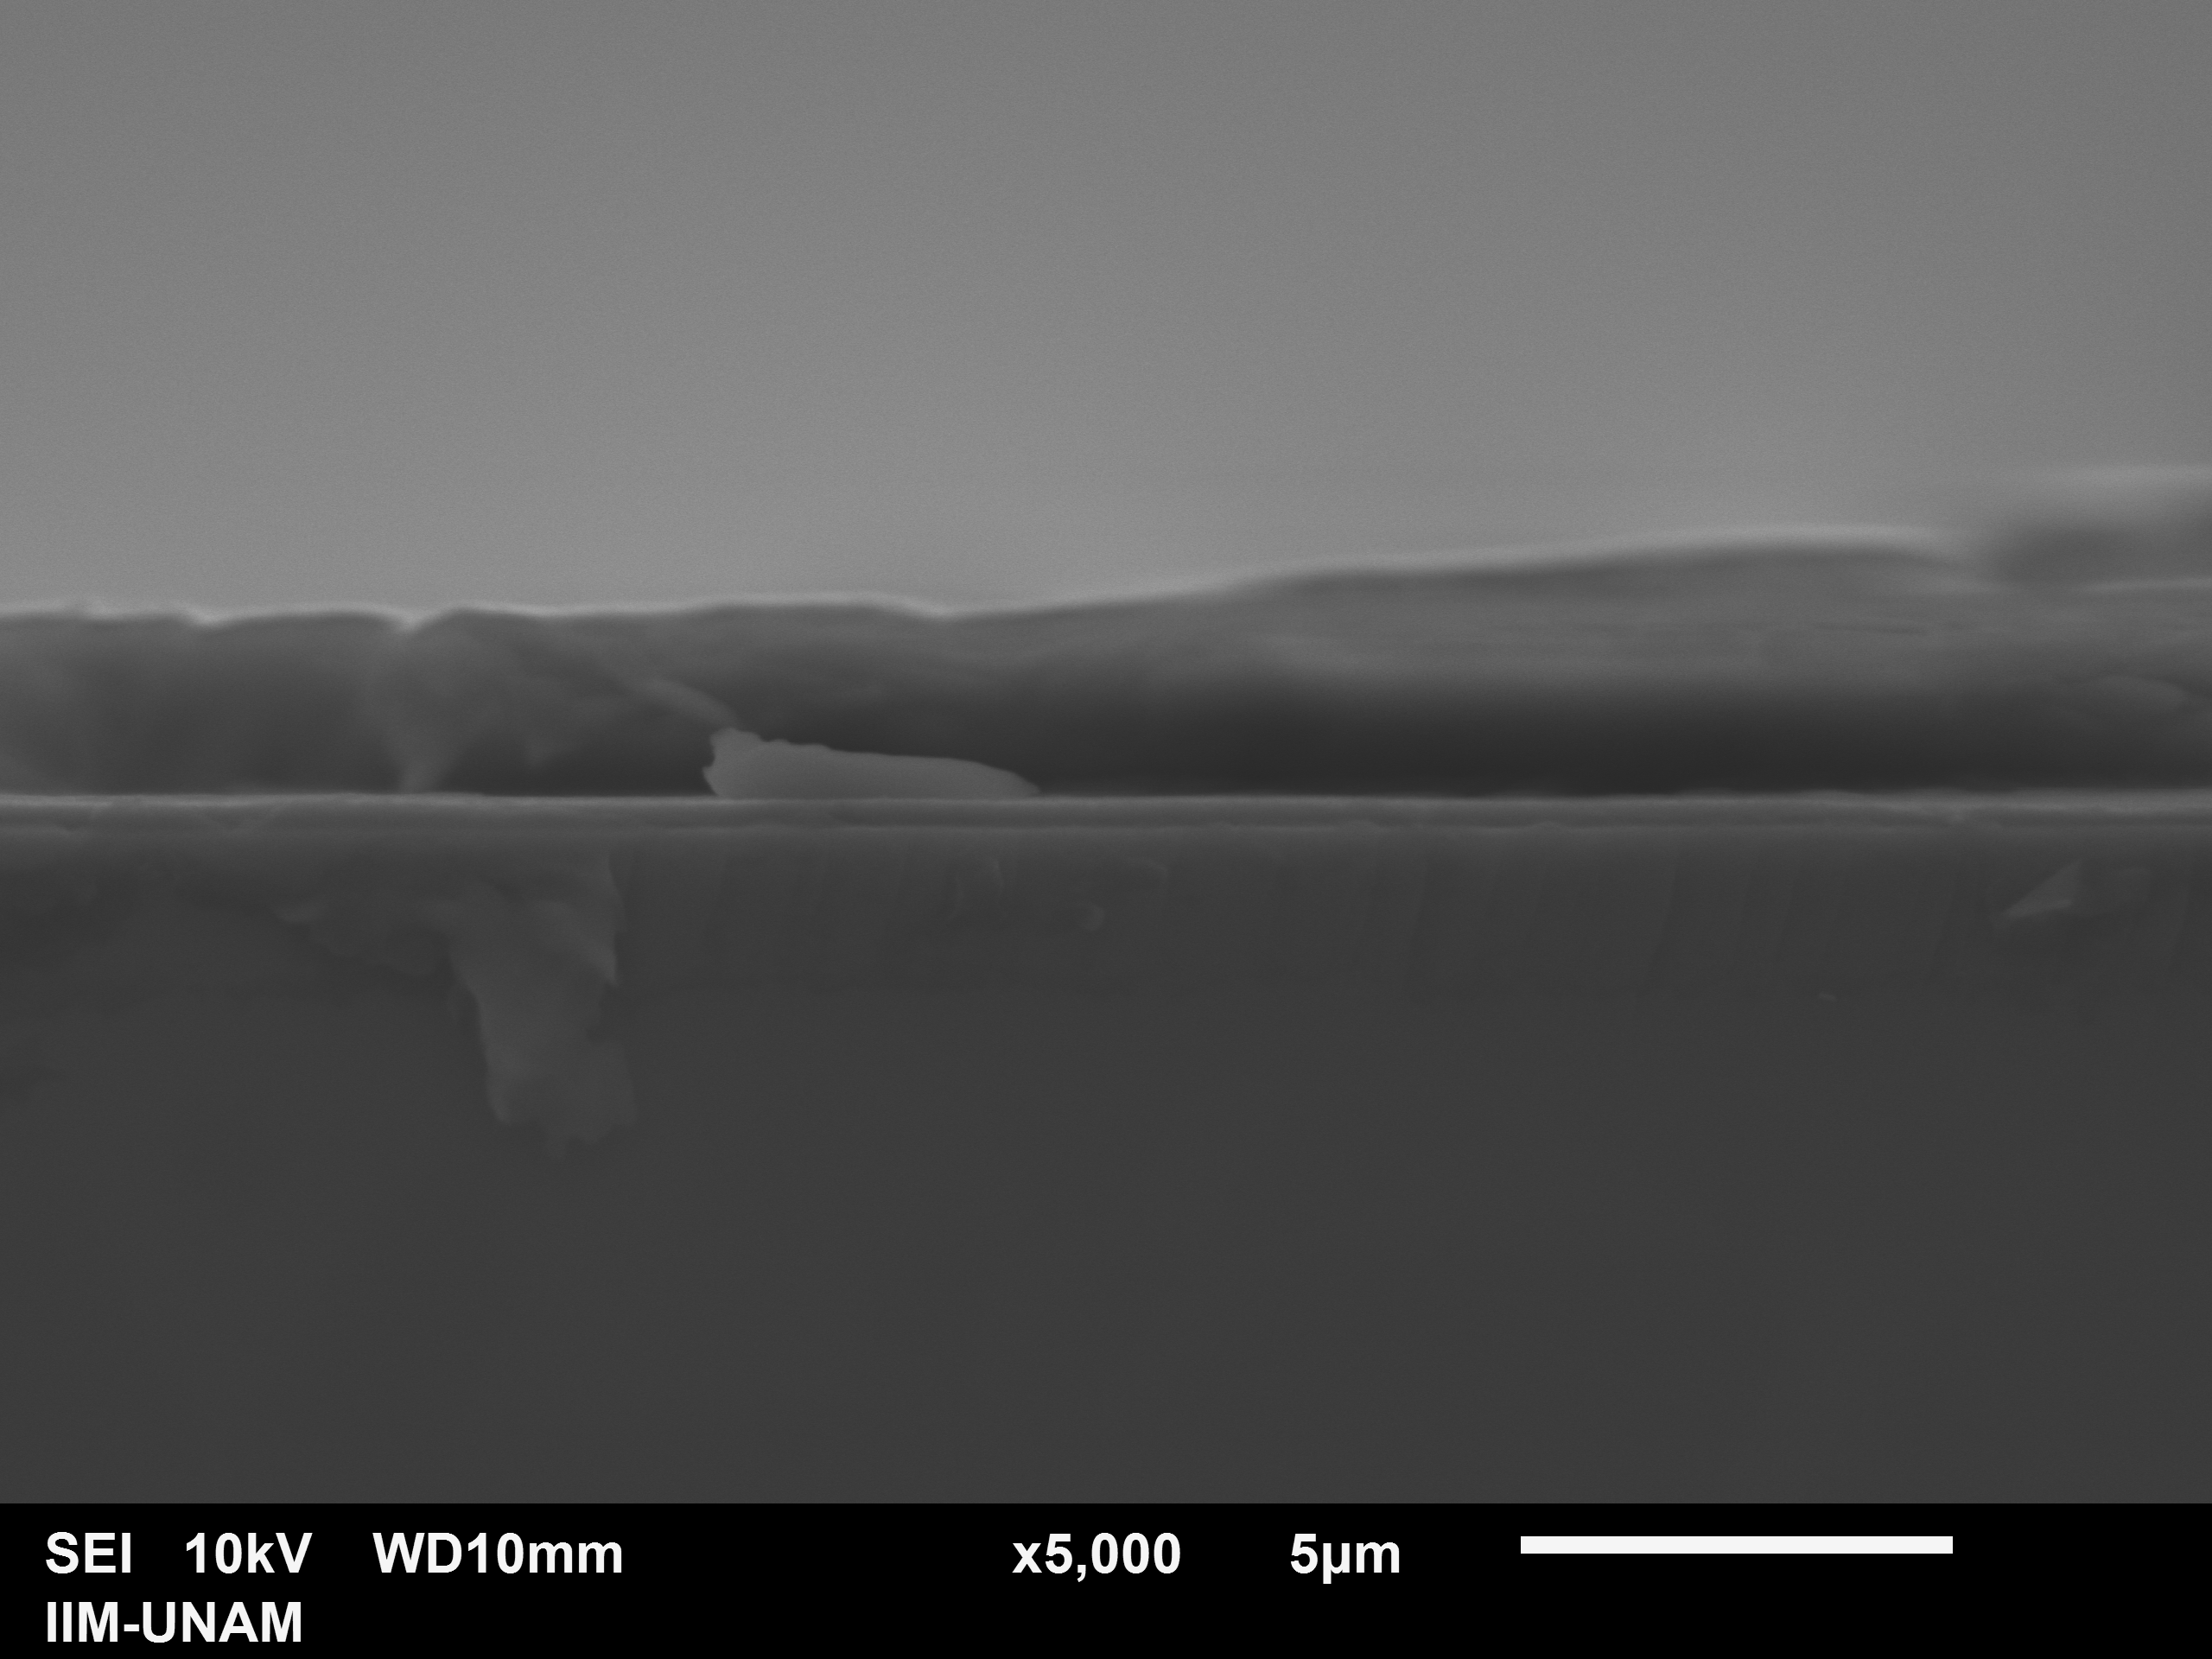
\includegraphics[width=\linewidth]{Al-transv-0008.png}
		\caption{Imagen de la sección transversal de la película de \ch{Al} observada con SE y en la que está presente el sustrato de \ch{Si}.}
	\end{subfigure}
	\caption{Imágenes de la sección transversal de la película de \ch{Al} depositada en el sustrato de \ch{Si}.}
	\label{fig:SEM-trans}
\end{figure*}

\begin{figure*}[ht]
	\centering
	\begin{subfigure}[b]{0.45\textwidth}
		\centering
		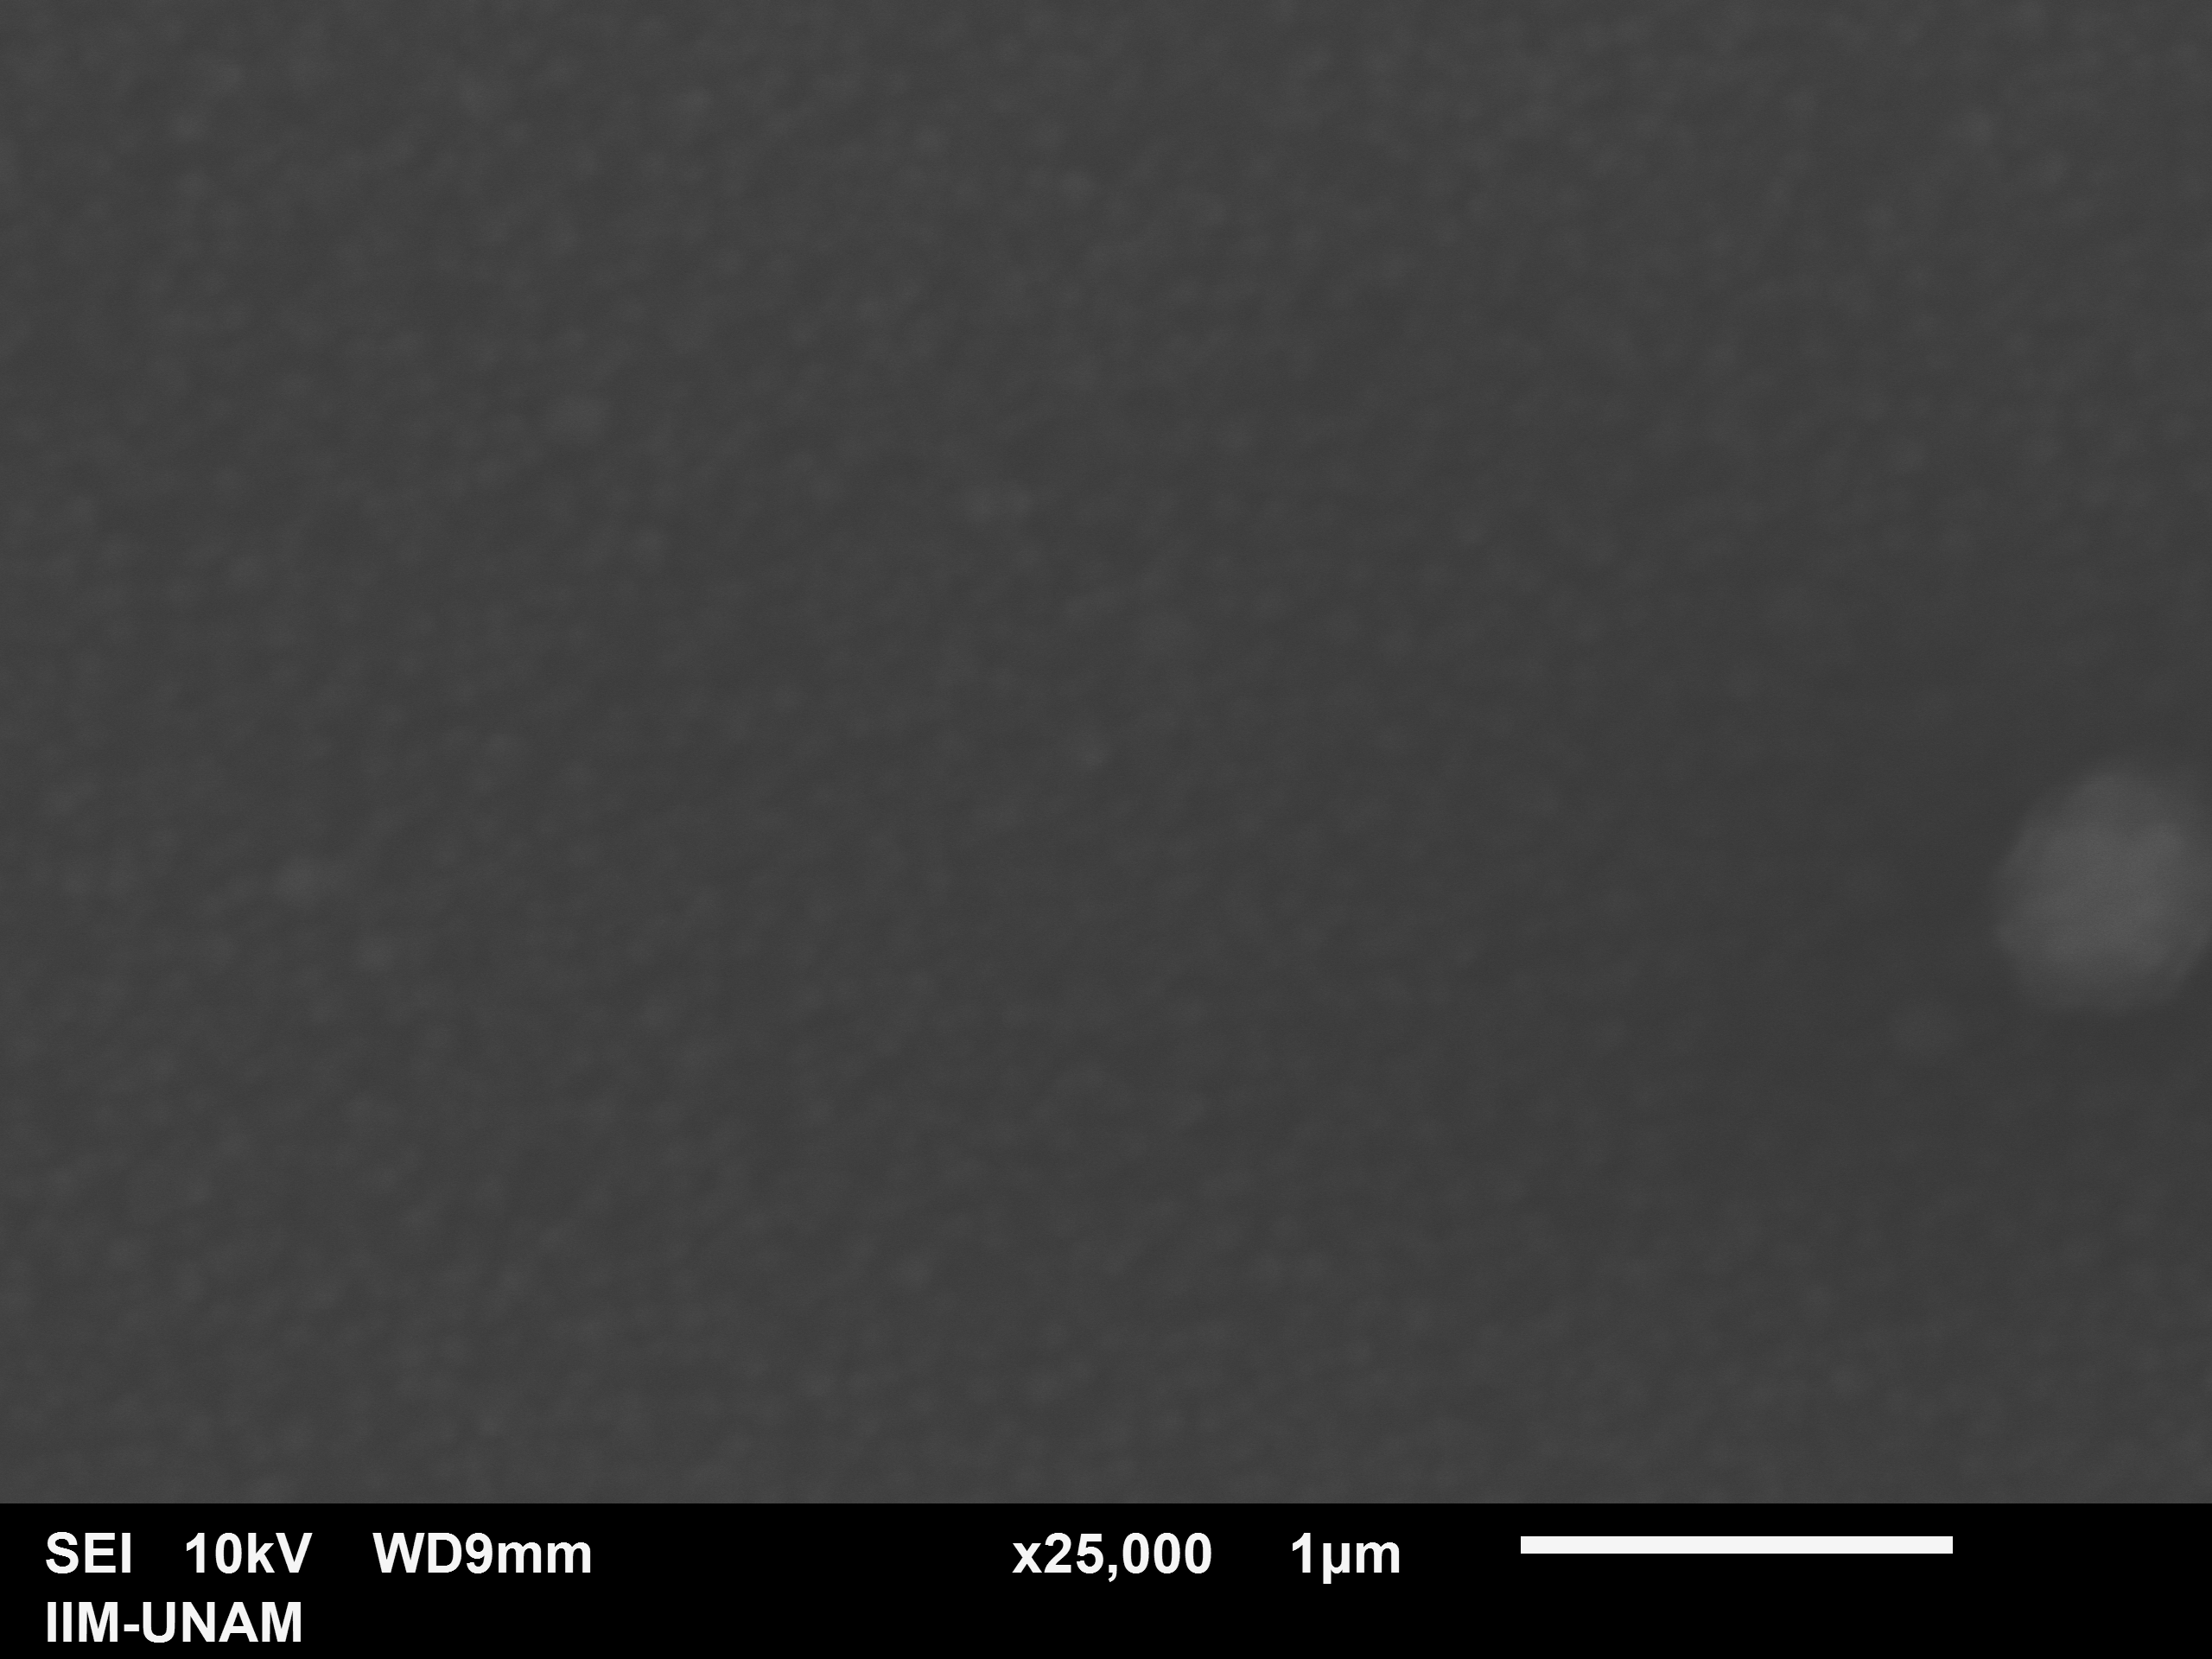
\includegraphics[width=\linewidth]{Al-sup-0001.png}
	\end{subfigure}%
	~
	\begin{subfigure}[b]{0.45\textwidth}
		\centering
		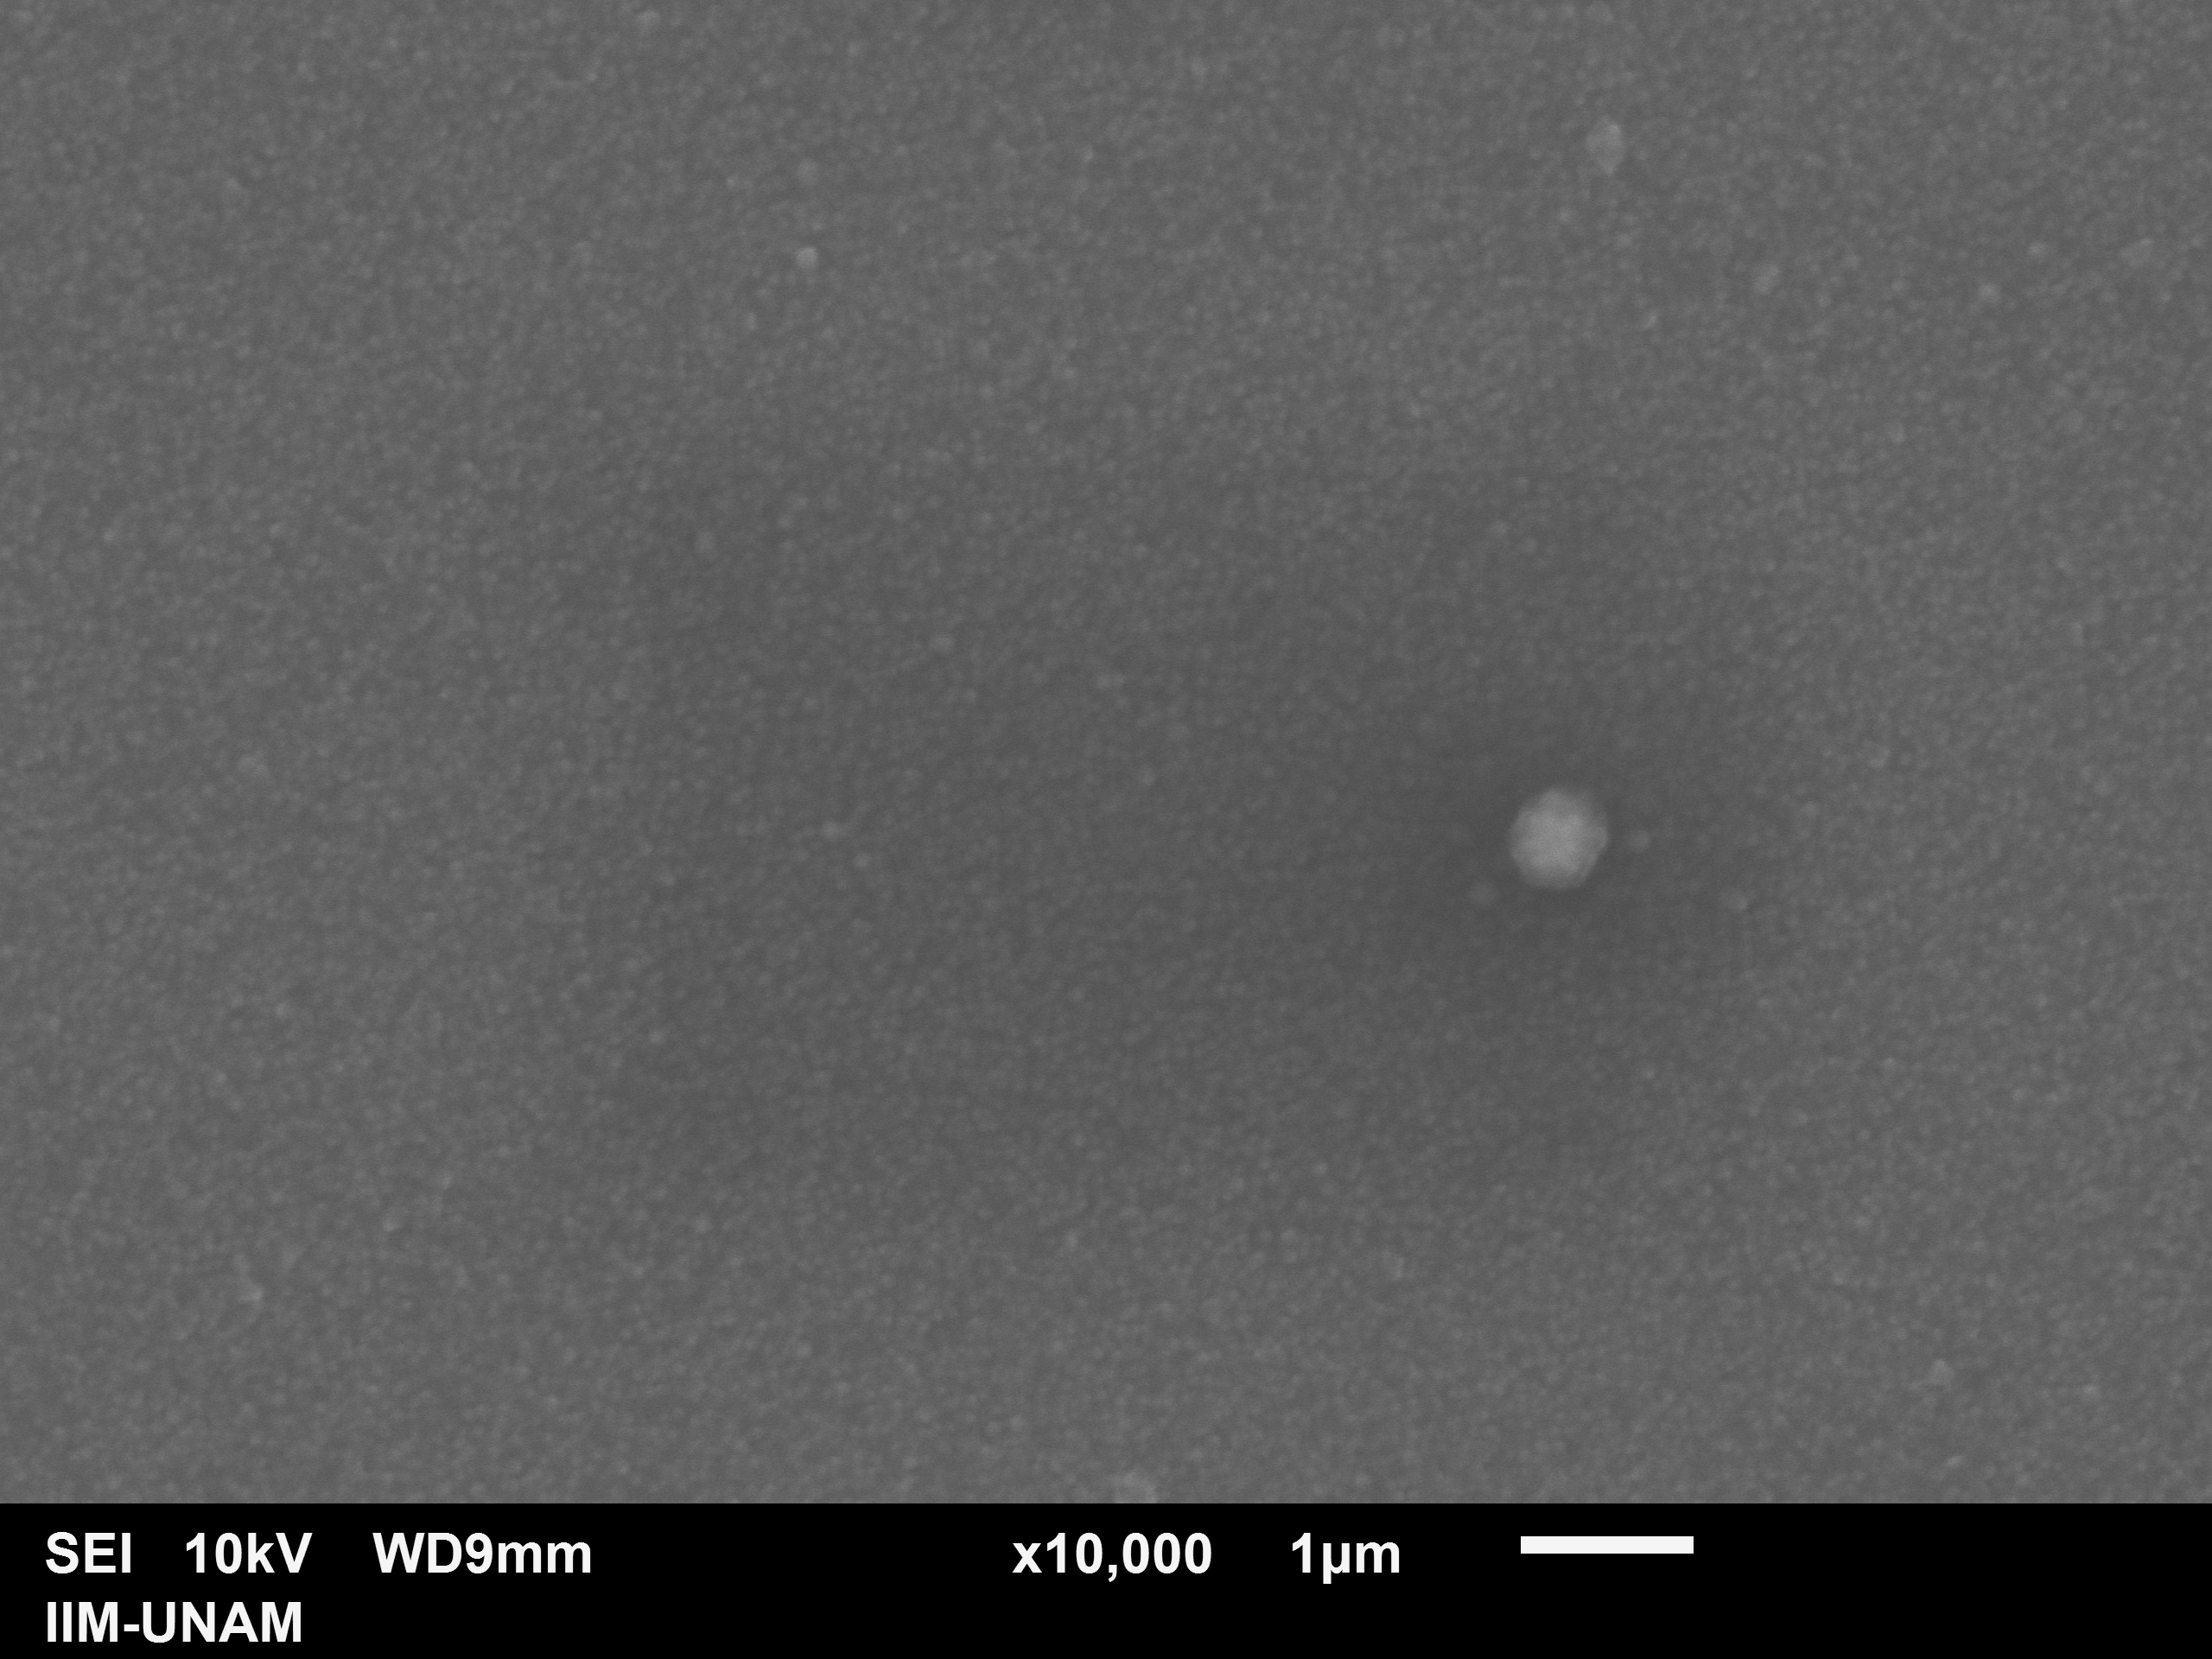
\includegraphics[width=\linewidth]{Al-sup-0002.png}
	\end{subfigure}
	\caption{Imágenes de la superficie de la película en la que se observa que el cremiento es granular.}
	\label{fig:SEM-superficie}
\end{figure*}

Otra prueba que nos puede ayudar a determinar la calidad de la película es la prueba de rayado (\emph{scratch}), la cual se encarga de evaluar entre otras cosas la adherencia de la película al sustrato. En este caso, se realizó la prueba de rayado en el portaobjetos de vidrio, donde se observó que la película se quedaba adherida al contracuerpo, lo que sugiere que la adherencia de la película al sustrato no es la adecuada o que la fuerza aplicada es demasiado alta.

Sin embargo, las imágenes obtenidas durante la prueba de \emph{scratch} no son suficientes para determinar la calidad de la película y analizar lo qué sucede a lo largo de la trayectoria de rayado. Por lo que se realizó un análisis de la fuerza de fricción en conjunto con las imágenes obtenidas de analizar la trayectoria de rayado en el perfilómetro óptico.

Por un lado, para la primera prueba de rayado, se observa que para el primer \qty{1}{\mm} la deformación que experimenta la película es plástica, ya que la fuerza de fricción no es la suficiente para desprender la película del sustrato. Sin embargo, que la película sea amorfa provoca cambios en la fuerza de fricción, lo que se traduce en picos significativo en la gráfica que se muetra de color rojo en \cref{fig:scratch-test-1}. En el resto de la trayectoria, la película se ha desprendido completamente del sustrato, lo cual provoca que la fuerza de fricción sea constante.

\begin{figure*}[htb]
	\centering
	% 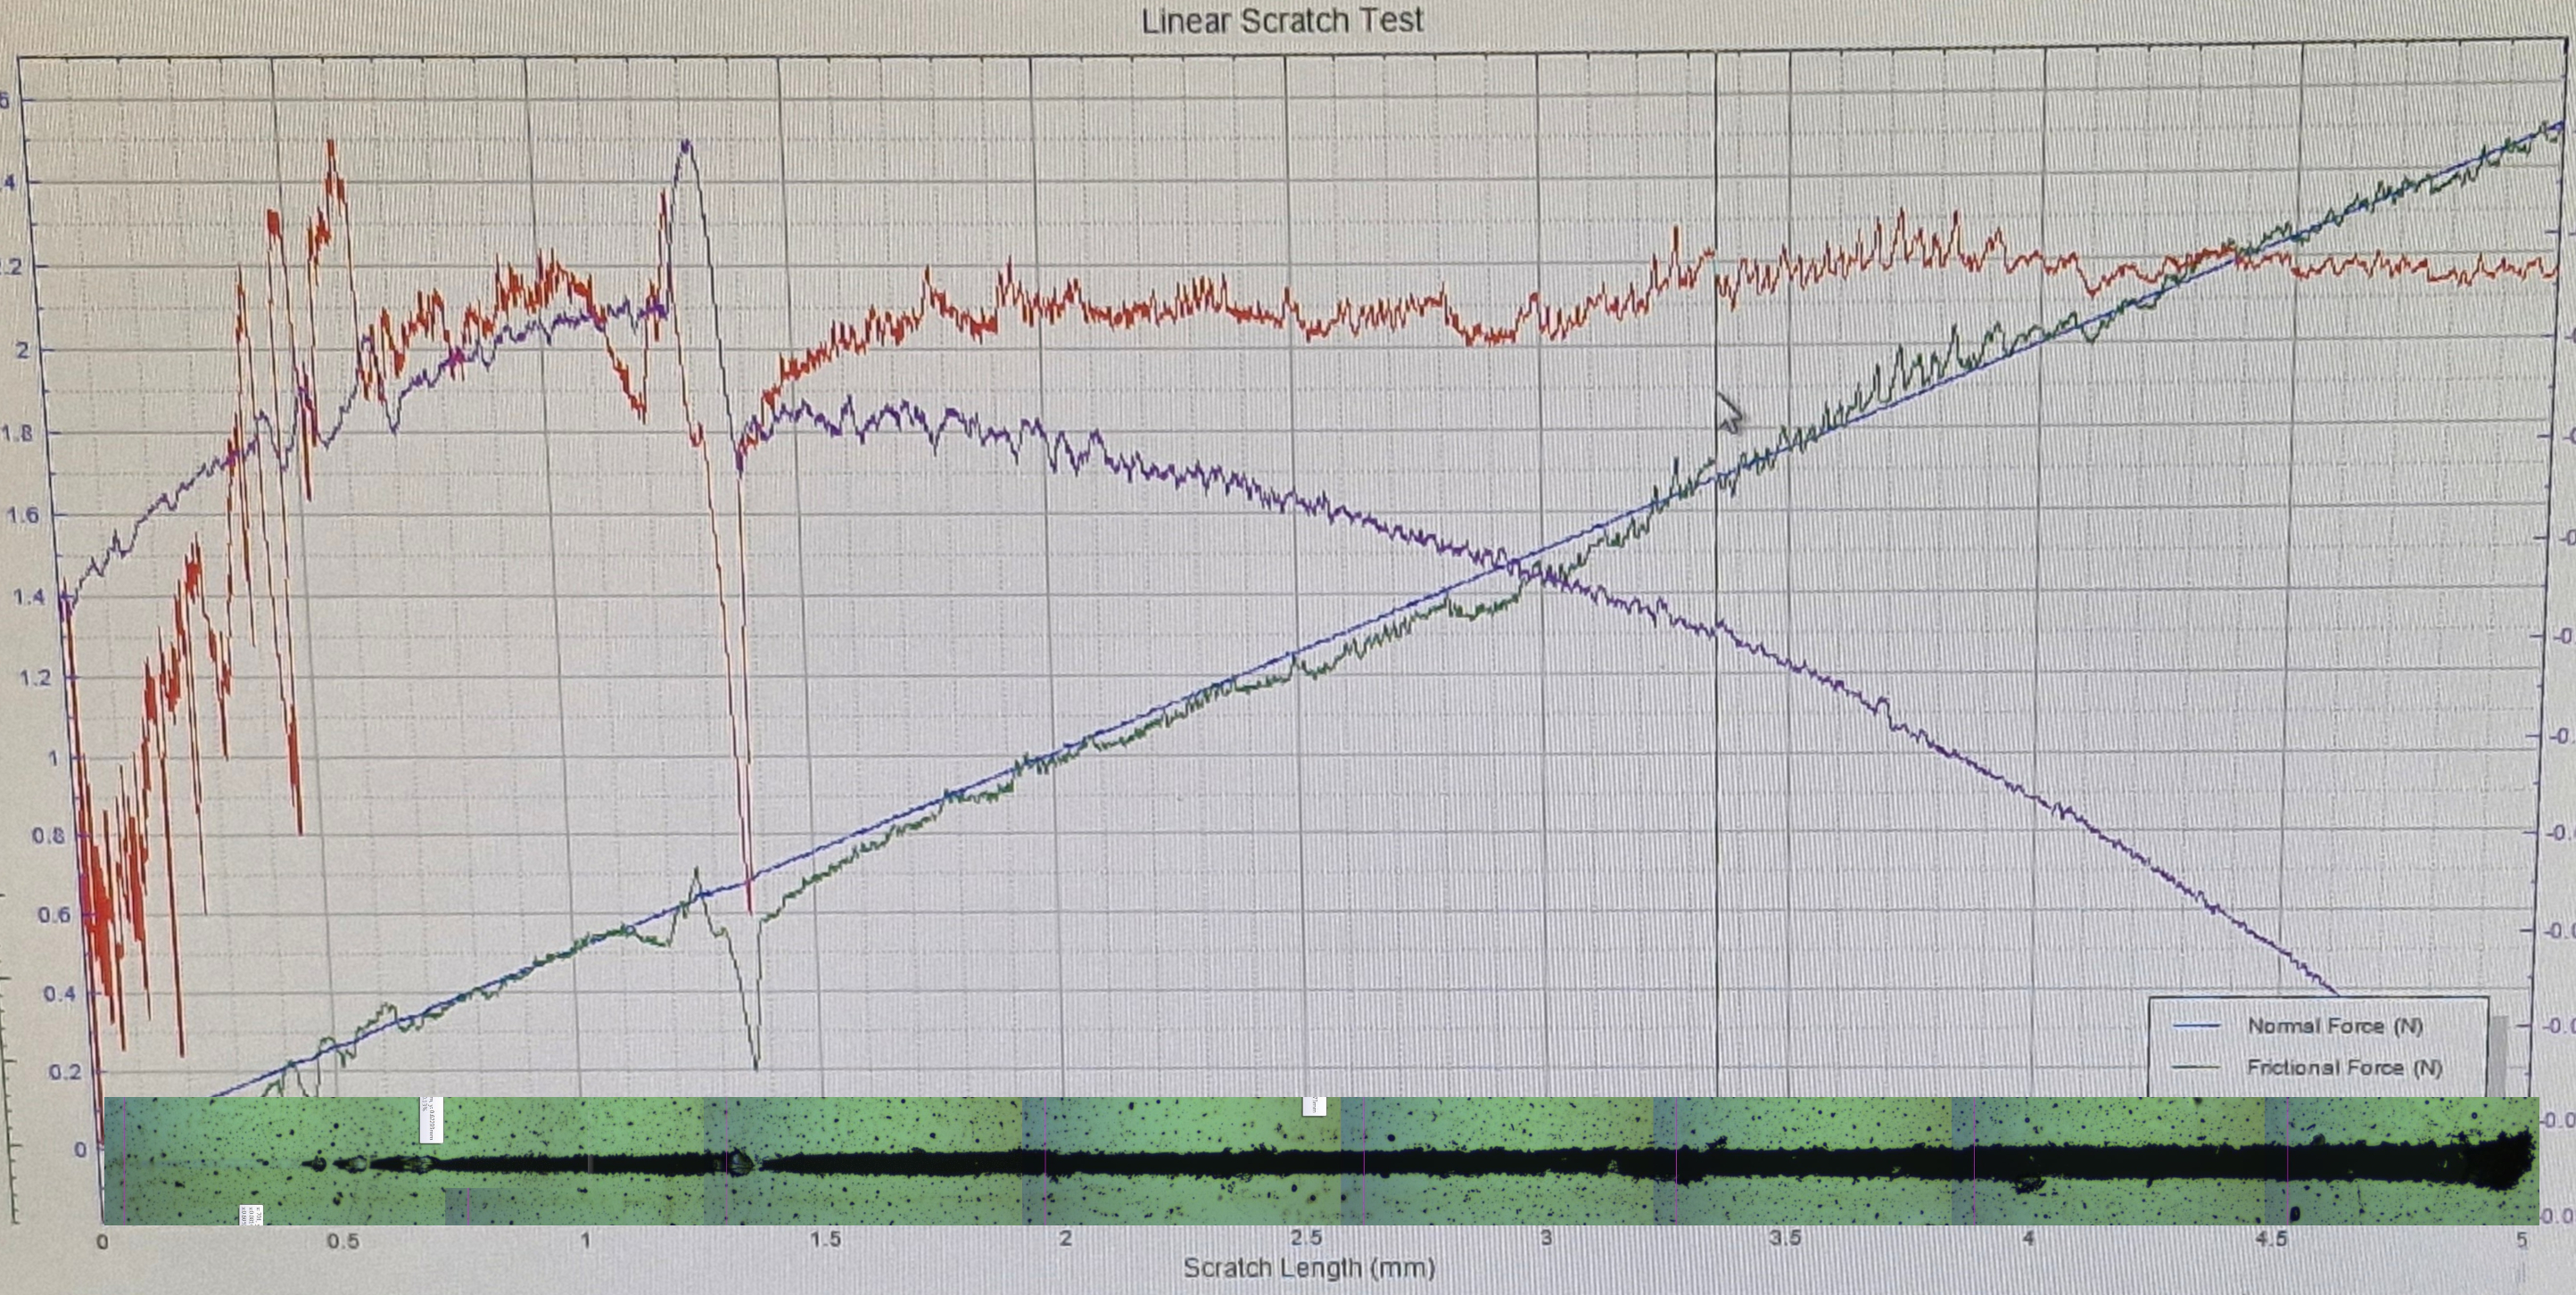
\includegraphics[width=\linewidth]{grafica-scratch_test_1}
	\includegraphics{example-image-a}
	\caption{Trayectoria de rayada para la prueba de \qty{0.1}{\N} hasta \qty{2.5}{\N}.}
	\label{fig:scratch-test-1}
\end{figure*}%

Para la segunda prueba de rayado, observamo el mimsmo tipo de comportamiento, en donde la película adherida al contracuerpo provoca un tipo de falla que no se esperaría para este tipo de película. En este caso, podríamos creer que la película presenta una falla del tipo Chevron, pero no es más que la presencia de impurezas debidas a la cámara de depósito. Nuevamente observamos un comportamiento casi constante de la fuerza de fricción (ver \cref{fig:scratch-test-2}), que nos indica que la película se ha desprendido completamente del sustrato.

\begin{figure*}[htb]
	\centering
	% \includegraphics[width=\linewidth]{grafica-scratch_test_2}
	\includegraphics{example-image-a}
	\caption{Trayectoria de rayada para la prueba de \qty{0.01}{\N} hasta \qty{1}{\N}.}
	\label{fig:scratch-test-2}
\end{figure*}

Estas deducciones del comportamiento observado durante la prueba de rayado se dedujó de las imágenes obtenidas del perfilómetro óptico, donde se observa que la parte de la trayectoria de color azul es la visualización del portaobjetos de vidrio, mientras que este mismo comporatmiento se observa de color verde en ciertas partes, pero representa lo mismo. Esto no es más que la consecuencia de la variación del espesor de la película.

\begin{figure}[htb]
	\centering
	\includegraphics[width=\linewidth]{OP-prueba_1-3D-path_final.jpg}
	\caption{Trayectoria de las dos pruebas de rayado en la que se observa el desprendimiento total de la película de \ch{Al} del sustrato de vidrio. De color verde ser observa la trayectoria debida a la primera prueba de rayado, mientras que de color azul se observa la trayectoria de la segunda prueba.}
\end{figure}

\section{Conclusiones}

Las películas delgadas de \ch{Al} depositadas por HiPIMS presentan un espesor promedio de \qty{280}{\nm}, por lo que la técnica de deposición elegida es la adecuada para la producción de películas delgadas. Sin embargo, se observó que la adherencia de las películas al sustrato no fue la adecuada, lo cual propicia la reflexión sobre el ajuste de los parámetros del depósito. Además es necesario plantearse \emph{a priori} el uso que se le dará a la película, ya que a partir de esta información se puede determinar el tipo de prueba tribológica a realizar, ya que en este caso la prueba de rayado no fue la más adecuada, pues el \ch{Al} es un material blando y se desprende con facilidad del sustrato, lo cual se ve reflejado en los resultados.

%%%%%%%%%%%%%%%%%%%%%%%%%%%%%%%%
%%%%%%    Bibliografia   %%%%%%%
%%%%%%%%%%%%%%%%%%%%%%%%%%%%%%%%
\pagebreak
\nocite{*}
\printbibliography
%\section{Apéndices}
%\appendices

\end{document}
%%%%%%%%%%%%%%%%%%%%%%%%%%%%%%%%
%%%%%% FIN DEL DOCUMENTO %%%%%%%
%%%%%%%%%%%%%%%%%%%%%%%%%%%%%%%%
